% Chapter 5

\chapter{Optimizing Wireless Sensor Networks} % Main chapter title
\label{Chapter5} % For referencing the chapter elsewhere, use \ref{Chapter2} 
\lhead{Chapter 5. \emph{Digital Signal Processor}} % This is for the header on each page - perhaps a shortened title
\textsf{\textsl{Written by Bjorn Deraeve}}
%----------------------------------------------------------------------------------------
\section{Introduction}
\subsection{What is digital signal processing?}
Signal processing falls within the scope of electrical engineering and applied mathematics that deals with the analysis of signals or operations on signals. In order to do this signals are presented in descrete time, discrete frequency or other discrete signal domains. The set of algorithmic solutions that are used to process digital signals are limited by the processing capabilities of the available hardware. 
Digital Signal Processing (DSP) algorithms have long been run on standard computers. Today additional technologies such as specialized processors called Digital Signal Processors (DSP) are used. DSP processors can  perform typical DSP operations more efficiently thanks to single-cycle multiply-accumulate (MAC) units, shift registers and extra large accumulators. To increase speed and possible DSP realizations DSP processors are used in purpose-built hardware such as application-specific integrated circuits (ASICs) or field-programmable gate arrays (FPGAs).

%----------------------------------------------------------------------------------------

\subsection{How are DSP processors used?}
DSPs receive real-world signals like voice, audio, video, ... that have been diditized and then mathematically manipulate them. DSP processors are a special type of microprocessors which are designed for performing mathematical functions like "add", "substract", "multiply" and "divide" very quickly.
Real-world analog signals are converted by Analog-to-Digital converters and are turned into the digital format of 0s and 1s. Now the DSP can start working on this digitized information. When all processing is done the new samples are mostly feed back in the real world via Digital-to-Analog converters. This whole process happens at very high speeds.\\
\begin{figure}[htbp]
\centering
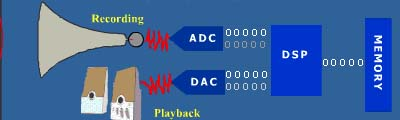
\includegraphics[height=3cm]{dspPrinciple}
\rule{30em}{0.5pt}
\caption{DSP Principle}
\label{fig:dspPrinciple}
\end{figure} \\
For our FM synthesizer application the first step is different. The DSP processing algorithms consist of algorithms that create the signal and signals that manipulate those signals so the AD converters on our FPGA are not used.

%----------------------------------------------------------------------------------------
\section{Digitization}  %sampling theorem
Real-world continuous signals have to be reduced to discrete signals (a numeric sequence) before a DSP can manipulate them. This sampling is done by an analog-to-digital converter (ADC) and the resulting samples are transported serially to the DSP.
\begin{figure}[htbp]
\centering
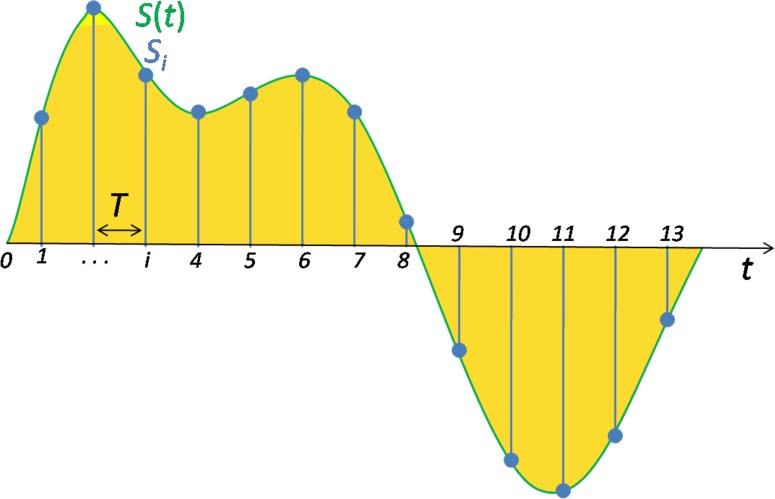
\includegraphics[height=3cm]{sampling}
\rule{30em}{0.5pt}
\caption{Signal sampling representation}
\label{fig:sampling}
\end{figure} \\
The sampling frequency $f_{s}$ is the number of samples taken in one second. According to the Nyquist criterion, the sampling frequency must at least be twice the frequency of the highest frequency component of interest. If the sampling frequency is greater than or equal to twice the bandwidth of a bandlimited signal then the signal can be (re)constructed without aliasing. This frequency is called the Nyquist rate. 
%----------------------------------------------------------------------------------------

\section{Digital Signal Processors}
As briefly mentioned in this chapter's introduction DSPs are processors with hardware, software, instruction sets, parallelism and data addressing that are optimized for high-speed numeric operations. 
A DSP contains the following key components:
\begin{itemize}
\item \textbf{Program Memory:} here the processing algorithms are stored
\item \textbf{Data Memory:} stores the signals to be processed
\item \textbf{Compute Engine:} performs the mathematical operations, coordinates access to program and data memory
\item \textbf{Input/Output:} connections to the outside world
\end{itemize}
\begin{figure}[htbp]
\centering
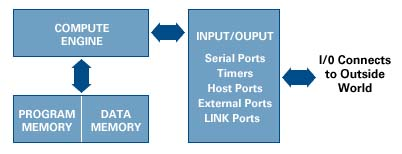
\includegraphics[height=2.5cm]{insideDSP}
\rule{30em}{0.5pt}
\caption[Structere of a DSP]{DSP structure}
\label{fig:insideDSP}
\end{figure} 
The need for high speed processors is because most DSP calculations are done on real-time signals. The inputsignal comes to the DSP as a train of individual samples from the AD converter. To do for example filtering in real-time, all calculations and operations on a sample must be completed before the next sample arrives. Usually also previous samples are needed so these must be stored somewhere and have to be quickly accesible. \\ 
%----------------------------------------------------------------------------------------
\subsection{Numeric architecture}
We know that DSPs must complete multiply-accumulate, additions and bit-shift operations in a single instruction cycle. Hardware optimized for such numeric operations is typical to DSP processors and distinguishes them from other general-purpose microprocessors.
The numeric operations are done by the DSP's MAC units, the arithmetic-logic unit (ALU) and barrel shifters:
\begin{itemize}
\item \textbf{MAC:} performs sum-of-products operations (used by FIR and IIR filters and fast Fourier transforms). The multiply-accumulate operation computes the product of two numbers and adds it to an accumulater:
\begin{equation}
a \shortleftarrow  a + ( b \times c )
\end{equation}
The multiplier is typically implemented in combinatonial logic followed by an adder and finally the accumulator register to store the result. If the output of the register is fed back to the adder each clock cycle the output of the multiplier is added to the register. Calculating multiplications with combinatorial logic requires a large amount of logic but is much faster than the method that uses shifts and additions.
\item \textbf{ALU:} performs standard addition, substraction and basic logical operations
\item \textbf{Barrel shifter:} performs operations on bits and words. This digital circuitry can shift a word by a specified number of bits in one clock cycle and is implemented as a sequence of multiplexers where the output of one mux is the input of the next mux. The input depends on the shift distance. An example of an 8-bit barrel shifter is shown in Figure \ref{fig:barrelShifter}. 
\begin{figure}[htbp]
\centering
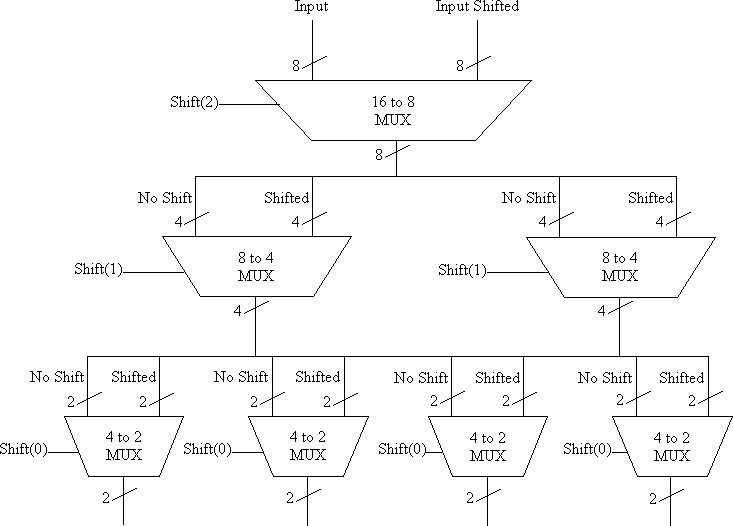
\includegraphics[height=6.5cm]{barrelShifter}
\rule{30em}{0.5pt}
\caption[8-bit Barrel Shifter]{8-bit barrel shifter}
\label{fig:barrelShifter}
\end{figure} \\
A barrel shifter is for example used for the implementation of floating-point arithmetic. To add two floats their significands must be aligned, which requires shifting the smaller number until it matches the exponent of the larger number.
\end{itemize}
As mentioned also parellelism plays a role in the efficiency of DSP processors. Figure \ref{fig:dspArchitecture} shows the parellelism of the ALU, MAC and shifter.
\begin{figure}[htbp]
\centering
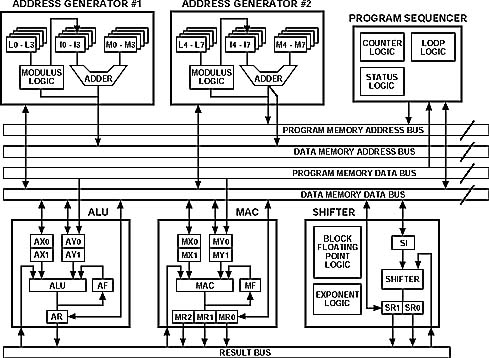
\includegraphics[height=6.0cm]{usefullDSPArchitecture}
\rule{30em}{0.5pt}
\caption[DSP architecture]{Useful DSP architecture}
\label{fig:dspArchitecture}
\end{figure}
%----------------------------------------------------------------------------------------
\subsection{Memory architecture}
Of course the memory of a DSP processor must be able to follow the high speed of the operations. Bus architecture must be optimized, there cannot be delays or bottlenecks. 
\begin{itemize}
\item Most general-purpose microprocessors use the von Neumann architecture and throughput is limited because of having to choose between either fetching data or fetching an instruction in each cycle. In DSP processors program memory and data memory have there own space and busses and can both be fetched in one cycle, doubling throughput. This structure is known as the Harvard architecture. Naturally additional optimizations  present on general-purpose processors, like instruction cache for example, are also present on DSPs.
\begin{figure}[htbp]
\centering
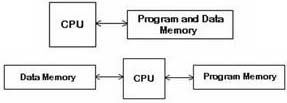
\includegraphics[height=2cm]{harvardVonNeuman}
\rule{30em}{0.5pt}
\caption[Harvard vs. Von Neuman]{Memory architecture: Von Neumann (top) vs. Harvard (below)}
\label{fig:harvardVonNeumann}
\end{figure}
\item A lot of DSP algorithms need to get data from memory in repeating patterns. For example the fetching and manipulation of samples stored in an array. By reducing instructions needed for memory access instruction cycles can be saved. To reduce this overhead DSPs use specialized data address-generators (DAG) to automatically manage these types of repeated memory accesses. 
Because most DSP algorithms use two operands the DSP has two DAGs. One address generator creates the address for the data memory bus, the other one for the program memory bus. By this way the DSP is able to sustain execution of instructions in one single cycle.
\item Often DSP algorithms require data in a range of addresses going from the end of the buffer back to the start of the buffer (wrap around). Therefore the DSP is provided with hardware circular buffers. The DAGs are specially designed for this task. General-purpose processors perform these functions in software and limit the ability to handle real-time signals.
\end{itemize}  
%----------------------------------------------------------------------------------------

\subsection{Sequencer architecture}
Since most algorithms runned on a DSP processor are by nature repetitive, the compute engine's program counter must be able to loop through the code without overhead while getting from the end of the loop back to the start. 
In general-purpose CPUs the loop's end condition is fully maintained in software. This condition instruction requires the fetching of addresses from memory and evaluation and takes time (cycles). DSP processors perform these tests in hardware, storing the needed addresses. In one cycle the condition is evaluated and either the first instruction of the loop is executed or the first instruction outside the loop is executed.
%----------------------------------------------------------------------------------------

\subsection{Input/Output architecture}
Because of the high data throuhput requirement of the DSP the whole design is focused on making data accessible for the numeric, memory and sequencer sections. To transfer data into and out of the DSP quickly serial communications and DMA is used. The use of serial communications above parallel is naturally since this way data is sended one bit at a time, following the DSPs operating frequency and distributing work load. So the DSP communicates with ADCs, DACs or other devices through synchronous serial ports (SPORT). Other functions such as timers and boot logic (in other words: hardware interrupts) also ease DSP system design. 
%----------------------------------------------------------------------------------------

\section{Fixed-point vs. floating-point DSP}
Digital signal processing can either be done with fixed point or with floating point data storage. DSPs designed to represent and manipulate integers are fixed point realizations. Floating-point DSPs represent and manipulate rational numbers. The number is represented in a similar manner to scientific notation, with a mantissa and an exponent (e.g. A $\times$ $2^{B}$ , where 'A' is the mantissa and 'B' is the exponent). 
\subsection{Advantages of floating-point digital signal processors}
In a fixed point DSP numbers are represented with a fixed number of digits after the decimal point, for example: 123.45, 1234.56, 12345,67, etc. In a floating point implementation the decimal point can 'float'.In addition a floating point representation can represent 1.234567, 123456.7, 0.001234567, etc.
Thanks to the exponential representation floating-point DSPs support a much larger dynamic range: very small numbers and very large numbers can be stored. Another advantage of this that floating-point processing yields much higher precision than fixed point processing.
\subsection{Considerations}
In digital signal processing rounding and/or truncating numbers yields quantization error or noise, a difference between the real-world value and the quantized digital values. This also happens each times a DSP does a mathematical calculation. As such, floating-point processors are the ideal DSP when accuracy is critical, like in audio applications. This is noticable in the program of our FM synthesizer, where constantly calculations are done with float data.
When choosing between fixed-point or floating-point processor there are many other important factors to consider, e.g. processor cost, ease of development, performance. In summary, because of the greater number of general purpose applications that can use fixed point processors those are typically less expensive than floating-point versions due to the scale of manufacturing. Floating-point DSPs are optimized for computationally intensive applications.
